\chapter{Results}\label{chapter:results}

In this chapter I present how my CUDA solution compares against the TensorFlow implementations of $\Phi_{Flow}$.
\par All benchmarks were performed in a closed boundary environment with random divergence vectors in the $\left[-1, 1 \right]$ range. The targeted residual accuracy was $1^{-5}$. Before starting the measurement, a warm-up of 5 runs was performed. The data shows the mean and standard deviation of 25 runs. The test system consists of a GeForce GTX 980, a Quad-Core Intel Core i7 3779K @3.5GHz CPU and 8GB of RAM.
\subsubsection{Performance Pressure Solve}
The following table shows the execution time per solve (t/s) and the average number of cg-iterations (iters) for quadratic grids and compares the Tensorflow solutions with my CUDA implementation: \\\\
\renewcommand{\arraystretch}{1.39}
\footnotesize{
\begin{tabular}{l||l|l|l|l|l|l||r|r}
\hline
\multirow{2}{*}{Dimension} & \multicolumn{2}{l|}{TF CPU} & \multicolumn{2}{l|}{TF GPU} & \multicolumn{2}{l||}{CUDA} & \multirow{2}{*}{Speedup CPU} & \multirow{2}{*}{Speedup GPU} \\ \cline{2-7} 
                  & t/s        & iters        & t/s        & iters        & t/s         & iters        &             &             \\ \hline
$64^2$   & 49,65 ms &  & 108,2 ms &  & 25,36 ms &  & 2.0 x   & 4.2 x  \\ \hline
$128^2$  & 207,6 ms &  & 396,3 ms &  & 39,49 ms &  & 5.3 x   & 10.0 x \\ \hline
$256^2$  & 1,169 s  &   & 1,839 s &  & 77,19 ms &  & 15.1 x  & 23.8 x \\ \hline
$512^2$  & 12,75 s  &   & 12,90 s &  & 240,9 ms &  & 52.9 x  & 53.6 x \\ \hline
$1024^2$ & 133.7 s  &   & 87,47 s &  & 1,412 s  &  & 94.6 x  & 61.9 x \\ \hline
$2048^2$ & n/a      &   & n/a     &  & 9,742 s  &  & n/a     & n/a    \\ \hline \hline

$64^3$   & 3,878 s  &  & 2,473 s  &  & 42,18 ms &  & 91.9 x  & 58.6 x \\ \hline
$128^3$  & 55.22 s  &  & 29,35 s  &  & 397,1 ms &  & 139.1 x & 73.9 x \\ \hline
$256^3$  & n/a      &  & n/a      &  & 5,814 s  &  & n/a  & n/a 		  \\ \hline
\end{tabular}
}

\begin{figure*}[t]
\centering
	\begin{subfigure}[b]{1\textwidth}
		\centering
		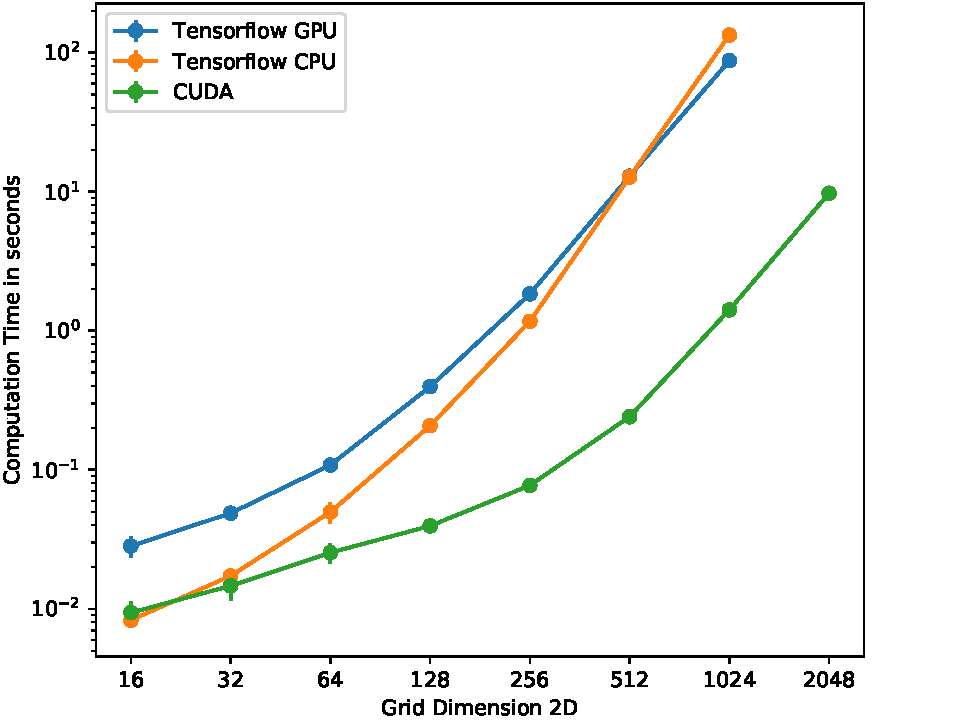
\includegraphics[height=9cm, width=14cm]{figures/performance_2d_bs1}

		\caption{Pressure Solve in 2D}
	\end{subfigure}
	\begin{subfigure}[b]{1\textwidth}
		\centering
		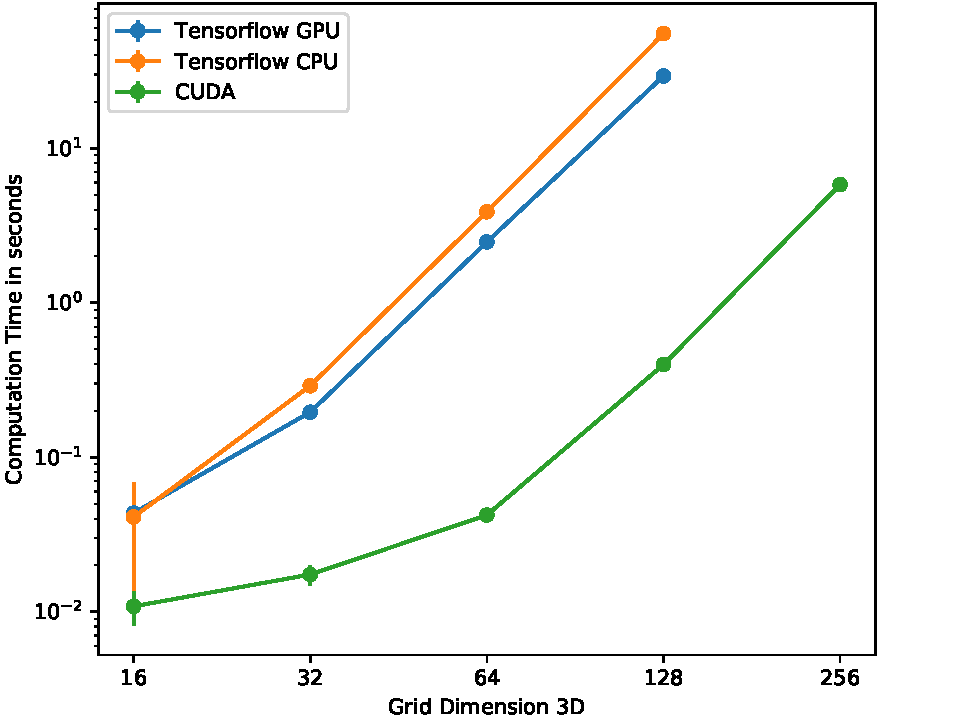
\includegraphics[height=9cm, width=14cm]{figures/performance_3d_bs1}

		\caption{Pressure Solve in 3D}
	\end{subfigure}

\caption{Execution time comparison between the three solvers and batch size 1.}	
\end{figure*}
